 \documentclass [12pt]{article} 

\usepackage {amsmath}
\usepackage {amsthm}
\usepackage {amssymb}
\usepackage {graphicx} 
\usepackage {float}
\usepackage {multirow}
\usepackage {xcolor}
\usepackage {algorithmic}
\usepackage [ruled,vlined,commentsnumbered,titlenotnumbered]{algorithm2e} \usepackage {array} 
\usepackage {booktabs} 
\usepackage {url} 
\usepackage {parskip} 
\usepackage [margin=1in]{geometry} 
\usepackage [T1]{fontenc} 
\usepackage {cmbright} 
\usepackage [many]{tcolorbox} 
\usepackage [colorlinks = true,
            linkcolor = blue,
            urlcolor  = blue,
            citecolor = blue,
            anchorcolor = blue]{hyperref} 
\usepackage {enumitem} 
\usepackage {xparse} 
\usepackage {verbatim}
\usepackage{listings}
\usepackage{xcolor}
\lstset { %
    language=C++,
    backgroundcolor=\color{black!5}, % set backgroundcolor
    basicstyle=\footnotesize,% basic font setting
}

\DeclareTColorBox {Solution}{}{breakable, title={Solution}} \DeclareTColorBox {Solution*}{}{breakable, title={Solution (provided)}} \DeclareTColorBox {Instruction}{}{boxrule=0pt, boxsep=0pt, left=0.5em, right=0.5em, top=0.5em, bottom=0.5em, arc=0pt, toprule=1pt, bottomrule=1pt} \DeclareDocumentCommand {\Expecting }{+m}{\textbf {[We are expecting:} #1\textbf {]}} \DeclareDocumentCommand {\Points }{m}{\textbf {(#1 pt.)}} 

\begin {document} 

{\LARGE \textbf {COMP 285 (NC A\&T, Spr `22)}\hfill \textbf {Lecture 3} } 
\vspace {1em} 
\begin {Instruction} 

Adapted From Virginia Williams' lecture notes. Additional credits: J. Su, W. Yang, Gregory Valiant, Mary Wootters, Aviad Rubinstein, Sami Alsheikh.
\end {Instruction} 

\begin{centering}
\section*{Asymptotics and Worst-Case Analysis}
\end{centering}


\section{Asymptotic Notation}
To talk about the running time of algorithms, we will use the following notation. $T(n)$ denotes
the runtime of an algorithm on input of size $n$.

\subsection{``Big-Oh'' Notation:}

Intuitively, Big-Oh notation gives an upper bound on a function. We say $T(n)$ is $O(f(n))$ when as $n$ gets big, $f (n)$ grows at least as quickly as $T(n)$. Formally, we say
$$
 T(n) = O(f(n)) \iff \exists c, n_0 > 0 \text{ s.t } \forall n \geq n_0, 0 \leq T(n) \leq c \cdot f(n)
$$

\subsection{``Big-Omega'' Notation:}

Intuitively, Big-Omega notation gives a lower bound on a function. We say $T(n)$ is $\Omega(f(n))$ when as $n$ gets big, $f (n)$ grows at least as slowly as $T(n)$. Formally, we say
$$
 T(n) = O(f(n)) \iff \exists c, n_0 > 0 \text{ s.t } \forall n \geq n_0, 0 \leq c \cdot f(n) \leq T(n)
$$

\subsection{``Big-Theta'' Notation:}

Intuitively, Big-Theta notation gives both a lower and upper bound on a function. We say $T(n)$ is $\Theta(f(n))$ if and only if $T(n) = O(f(n))$ and $T(n) = \Omega(f(n))$.
$$
 T(n) = O(f(n)) \iff \exists c_1, c_2, n_0 > 0 \text{ s.t } \forall n \geq n_0, 0 \leq c_1 f(n) \leq T(n) \leq c_2 f(n)
$$

We can see that these notations really do capture exactly the behavior that we want - namely, to focus on the rate of growth of a function as the inputs get large, ignoring constant factors and lower order terms. As a sanity check, consider the following example and non-example.

\begin{figure}[ht!]
\centering
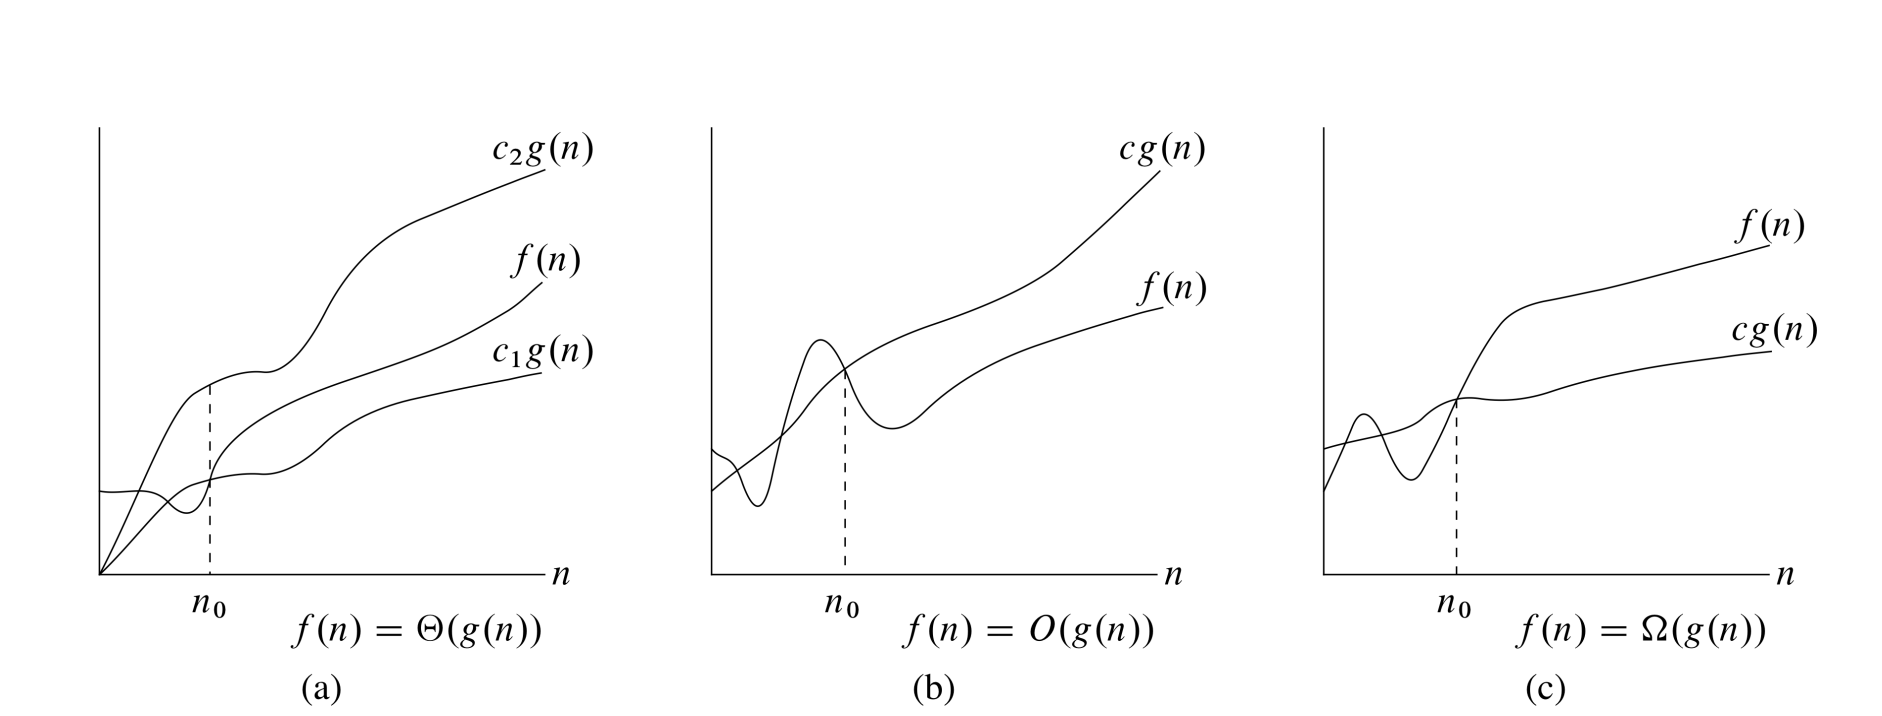
\includegraphics[scale=0.4]{asymptotics.png}
\caption{Figure 3.1 from CLRS - Examples of Asymptotic Bounds. (Note: In these examples, $f(n)$ corresponds to our $T(n)$ and $g(n)$ to our $f(n)$).}
\label{fig:example}
\end{figure}

\textbf{Claim 1.} \textit{All degree-$k$ polynomials\footnote{To be more precise, all degree-$k$ polynomials $T$ such that $T(n) \geq 0$ for all $n \geq 1$. How would you adapt this proof to be true for all degree-$k$ polynomials $T$ with positive leading coefficients?} are $O(n^k)$.}
\textit{Proof.} Suppose $T(n)$ is a degree-$k$ polynomial. That is, $T(n) = a_k n^
k + \dots + a_1n + a_0$ for some choice of $a_i$'s where $a_k \neq 0$. To show that $T(n)$ is $O(n^k)$ we must find a $c$ and $n_0$ such that for all $n \geq n_0, T(n) \leq c \cdot n^k$. (Since $T(n)$ represents the running time of an algorithm, we assume it is positive.) Let $n_0 = 1$ and let $a^* = max_i|a_i|$. We can bound $T(n)$ as follows:
\begin{align*}
T(n) &= a_kn^k + \dots + a_1n + a_0 \\
&\leq a^*n^k + \dots + a^*n + a^* \\
&\leq a^*n^k + \dots + a^*n^k + a^*n^k \\
= (k+1)a^*\cdot n^k
\end{align*}
Let $c = (k+1)a^*$ which is constant, independent of $n$. Thus, we've exhibited $c, n0$ which satisfy the Big-Oh definition, so $T(n) = O(n^k)$.

\textbf{Claim 2.} \textit{For any $k \geq 1$, $n^k$ is not $O(n^{k-1})$}.
\textit{Proof.} By contradiction. Assume $n^k = O(n^{k-1})$. Then there is some choice of $c$ and $n0$ such that $n^k \leq c \cdot n^{k-1}$ for all $n \geq n_0$. But this in turn means that $n \leq c$ for all $n \geq n_0$, which contradicts the fact that $c$ is a constant, independent of $n$. Thus, our original assumption was false and $n^k$
is not $O(n^{k-1})$.

\section{MergeSort}
Recall the \textit{Divide-and-conquer} paradigm from the second lecture. In this paradigm, we use the following strategy:

\begin{itemize}
    \item Break the problem into sub-problemsn.
    \item Solve the sub-problems (often recursively)
    \item Combine the results of the sub-proboems to solve the big problem.
\end{itemize}

At some point, the sub-problems become small enough that they are easy to solve, and then we can stop recursing.

With this approach in mind, \texttt{MergeSort} is a very natural algorithm to solve the sorting problem.

The pseudocode is below:

\begin{verbatim}
MergeSort(A):
    n = len(A)
    if n <= 1:
        return A
    L = MergeSort( A[:n/2] )
    R = MergeSort( A[n/2:] )
    return Merge(L, R)
\end{verbatim}

Above, we are using Python notation, so $A[: n/2] = [A[0], A[1], \dots , A[n/2 - 1]]$ and $A[n/2 :] = [A[n/2], . . . , A[n - 1]]$. Additionally, we're using integer division, so n/2 means $\lfloor n/2 \rfloor$.

How do we do the \texttt{Merge} procedure? We need to take two sorted arrays, $L$ and $R$, and merge them into a sorted array that contains both of their elements. See the slides for a walkthrough of this procedure.

\begin{verbatim}
Merge(L, R):
    m = len(L) + len(R)
    S = [ ]
    for k in range(m):
        if L[i] < R[j]:
            S.append( L[i] )
            i += 1
        else:
            S.append( R[j] )
            j += 1
    return S
\end{verbatim}

\textbf{Note:} This pseudocode is incomplete! What happens if we get to the end of $L$ or $R$? Try to adapt the pseudocode above to fix this.

As before, we need to ask: Does it work? And does it have good performance?

\end{document}